\documentclass[12pt]{article}
\usepackage[utf8]{inputenc}
\usepackage{amsmath}
\usepackage{amsfonts}
\usepackage{amssymb}

% this is to make it look like a word document.
\usepackage[tmargin=0.98in,bmargin=0.98in,lmargin=1.18in,rmargin=1.18in]{geometry}

% package necessary to add pictures to latex
\usepackage{graphicx}

\title{\vspace{-2ex}Enfoque basado en fronteras para exploración autónoma\vspace{-2ex}}
\date{\today}
\author{Luis Servín\\ Taller TRA, Universidad Nacional Autónoma de México}

\begin{document}

\maketitle

\section*{Resumen}

Se presenta un nuevo enfoque basado en el concepto de fronteras, las cuales se pueden definir como el límite entre una región conocida abierta y un espacio aún sin explorar. Al moverse a las distintas fronteras dentro de su mapa un robot puede expandir su conocimiento del ambiente que lo rodea. 

El método presentado se basa en los mapas de cuadrícula (evidence grid) y la navegación hacia estas fronteras. Una de las principales ventajas de este método es su capacidad de explorar tanto amplios sitios abiertos como espacios estrechos desordenados.

\section{Introducción}

Usualmente un mapa para uso humano debe proveer ya sea la localización exacta de los obstáculos (mapas métricos) o de una manera gráfica las formas de conexión entre reqiones abiertas (mapas topológicos). 

Se define el término \textbf{exploración} como la acción de moverse a través de un ambiente desconocido mientras se construye un mapa que puede ser utilizado como base de un sistema de navegación. Por lo tanto una buena estrategia de exploración generará un mapa completo o casi completo de una zona en una cantidad de tiempo razonable.

Aunque durante las simulaciones frecuentemente se ve al mundo como un conjunto de planos. Un robot móvil real tendrá que navegar a través de espacios desordenados, donde las paredes pueden estar escondidas detrás de escritorios o libreros.

Solo unas pocas investigaciones de sistemas de navegación usados en ámbitos reales han sido hechos. Algunos ejemplos son sistemas de exploración limitados a ambientes que pueden ser explorados usando seguimiento de paredes, mientras que otros requieren que las paredes se intersecten en ángulos rectos o que dichas paredes no se encuentren obstruidas y sean visibles para el robot.

Por lo tanto nuestro objetivo es desarrollar una estrategia de exploración para ambientes complejos como los que se encuentran típicamente en ambientes de oficina. Esta estrategia se basa en la detección de fronteras, regiones sobre el límite entre espacios abiertos conocidos y regiones sin explorar.

\section{Exploración Basada en Fronteras}

La pregunta central dentro de la exploración es: Dado lo que conoces acerca del mundo \textbf{¿Hacia que dirección deberías moverte para obtener la mayor cantidad de información posible?} Dado que en un inicio no se tiene conocimiento previo del ambiente mas allá de la información que se puede obtener del punto en el que te encuentras.

La idea central detrás de la exploración basada en fronteras es: Obtener la mayor cantidad de información nueva acerca del mundo como consecuencia de desplazarse hacia una de las fronteras conocidas.

\textbf{Frontera}: Región en el límite entre un territorio conocido abierto y un espacio aún sin explorar. Por lo tanto al moverse hacia una frontera un robot obtiene nueva información acerca del ambiente. Realizando esta acción de manera repetitiva le permite incrementar su conocimiento del ambiente que lo rodea.

Un robot que cuenta con un mapa perfecto podría navegar a cualquier punto en dentro del espacio, y por lo tanto ese punto se considera accesible. Todos lo puntos accesibles son continuos ya que debe existir una ruta entre ellos debe existir. 

De esta manera, un robot que hace uso de la exploración basada en fronteras habrá de explorar todas las regiones accesibles dentro de su mundo, asumiendo el uso de sensores y sistemas de odometría perfectos.

Pero la pregunta real sería ¿Cuál sería el desempeño de la estrategia de navegación basada en fronteras al trabajar con sensores que son afectados por ruido y un control imperfecto de los motores en un mundo real?

\section{Detección de fronteras}

Cada celda dentro de nuestro mapa de cuadrículas puede ser clasificada al comparar la probabilidad de que se encuentre ocupada con la probabilidad inicia asignada (Generalmente se aplica una probabilidad inicial de 0.5). Por lo tanto cada celda se puede encontrar en alguna de estas tres categorías:

\begin{itemize}
	\item \textbf{abierta}: Probabilidad de ocupación $<$ Probabilidad inicial
	\item \textbf{desconocida}: Probabilidad de ocupación $=$ Probabilidad inicial
	\item \textbf{ocupada}: Probabilidad de ocupación $>$ Probabilidad inicial
\end{itemize}

\begin{figure}[!h]
	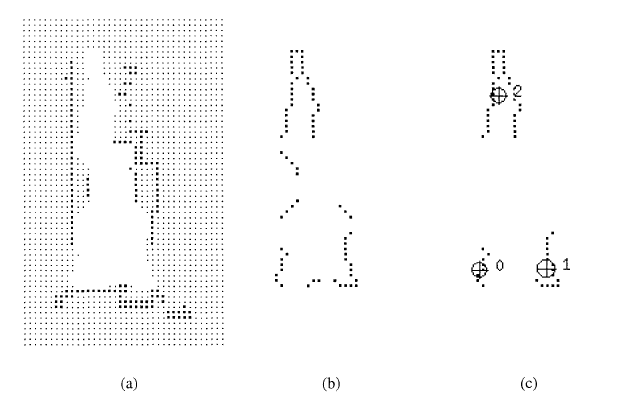
\includegraphics[scale=1]{images/frontier_detection.PNG}
	\caption{Detección de la frontera}
	\label{fig:frontier1}
\end{figure}

Cualquier celda abierta conocida adyacente a una celda desconocida es etiquetada como una \emph{celda de borde de frontera}. Celdas de borde de frontera son agrupadas en \emph{regiones de frontera}. Mientras que las regiones de frontera que cumplan con un tamaño mínimo (Cercano al tamaño del robot) son consideradas \textbf{fronteras}.

\section{Navegando hacia las fronteras}

Una vez que las fronteras han sido detectadas, el robot intentará navegar hacia la frontera más cercana y accesible que no haya sido visitada aún. Para lograr este objetivo se hace uso de un algoritmo de planeación de ruta, para llegar a la ubicación seleccionada a través de un camino libre de obstáculos.

Durante el recorrido, se hace uso de un comportamiento reactivo de evasión de obstáculos, el cual evite que el robot colisione con algún obstáculo que no fue previsto durante la planeación de ruta. Este comportamiento le permite al robot evadir un obstáculo imprevisto, y regresar a la ruta planeada inicialmente siempre y cuando no hayan ocurrido cambios muy drásticos en su entorno.

Una vez que el robot ha alcanzado el punto objetivo dentro de mapa se marca la zona como conocida dentro del mapa. Enseguida se realiza un giro de 360 grados ya sea solamente del sensor o del sistema completo con el objetivo de añadir mas información acerca del entorno. Con la información obtenida se actualiza el mapa del entorno. Una vez actualizado el mapa se repite el proceso con una nueva frontera como objetivo.

Si se presenta el caso de que el robot no pueda llegar a su destino después de una cierta cantidad de tiempo, se establece dicho objetivo como inaccesible y se procede con a alguna otra frontera que aún quede disponible.

\section{Experimentos}

El experimento se llevo a cabo utilizando una plataforma \emph{Nomad 200} equipada con un sensor laser, dieciseis sonares, y dieciseis sensores infrarrojos. La totalidad de los sensores infrarrojos y sonares fueron utilizados para la evasión de obstáculos. Se cuenta con un sistema de procesamiento \emph{Sparcstation}. Mientras que la comunicación es realizada por medio de un sistema de radio-ethernet.

Se llevaron a cabo dos experimentos en ambientes reales de oficina. El primer ambiente incluía sillas, escritorios, mesas, libreros, gabinetes, muebles, un enfriados de agua y cajas de distintos tamaños y formas.

En la figura \ref{fig:small_office_map} se muestran los resultados después de un intento.

\begin{figure}[ht]
	\centering
	\begin{minipage}[b]{0.45\linewidth}
		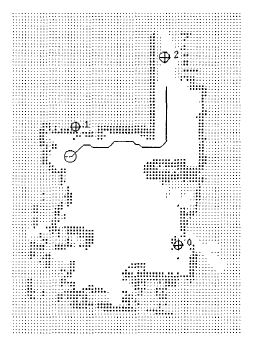
\includegraphics{images/small_office.JPG}
		\caption{Espacio de oficina pequeño}
		\label{fig:small_office_map}
	\end{minipage}
	\quad
	\begin{minipage}[b]{0.45\linewidth}
		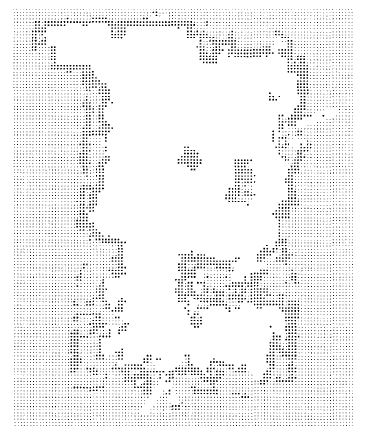
\includegraphics{images/large_office.JPG}
		\caption{Espacio de oficina grande}
		\label{fig:large_office_map}
	\end{minipage}
\end{figure}

Aquellas celdas con baja probabilidad se encontrarse ocupadas son representadas con un espacio en blanco, las que no se conoce su probabilidad con puntos pequeños, mientras que las celdas con altas probabilidades de estar ocupadas con puntos mas grandes. La posición del robot se representa a través de un círculo negro con un línea central que muestra la orientación del robot.

El tiempo total requerido para completar este mapa fue de alrededor de media hora. Una versión mejorada de este algoritmo demostró poder realizar la tarea en alrededor de 15 minutos.

El segundo experimento se realizó en un espacio de oficina mucho mas amplio. en la figura \ref{fig:large_office_map} se muestra el mapa obtenido.

Aunque el área total fue mayor, el robot fue capaz de completar el espacio en alrededor de media hora. Esto puede deberse a la gran cantidad de espacios libres que se encuentran.

\section{Conclusiones y Trabajo a Futuro}

Un robot que hace uso de la exploración basada en fronteras presenta las siguientes ventajas:

\begin{itemize}
	\item Puede explorar una amplía variedad de ambientes, ya sea que tengan amplios espacios abiertos o zonas congestionadas y reducidas.
	\item Las paredes y los obstáculos dentro del espacio a explorar no tienen que cumplir con alguna orientación específica.
	\item La eficiencia aumenta al hacer que el robot se mueva hacia los lugares a los cuales tiene mayor probabilidad de obtener nueva información.
\end{itemize}.

Actualmente se desarrollo un experimento en el cualquier se combina las capacidades del sistema de exploración basado en fronteras con técnicas de localización, logrando obtener obtener resultados muy esperanzadores.

% commands for using bibliography and citations 
%\bibliographystyle{ieeetr}
%\bibliography{bibliography}

\end{document}























